\documentclass[12pt]{ctexart}
\usepackage{amsmath,graphicx,textcomp,subfigure,indentfirst,ctex,color,float}
\usepackage{bm, mhchem}
\title{Lecture 13}
\author{授课、校对:茅奕  \\ 记录:赵思逸}

\date{2022年5月31日}

\newcommand{\refeq}[1]{式~(\ref{#1})}
\newcommand{\refeqs}[2]{式~(\ref{#1}) - (\ref{#2})}
\newcommand{\reffig}[1]{图~\ref{#1}}
\begin{document}

\maketitle





\section{盘星系的形成}

盘星系 (Disk Galaxy) 有盘结构,有些有旋臂,有些有棒状结构。
它的主要亮度集中在盘面上,但一般盘面两侧也有恒星和气体,
单纯只有盘的星系非常少。

\begin{figure}[!hbtp]
	\centering 
	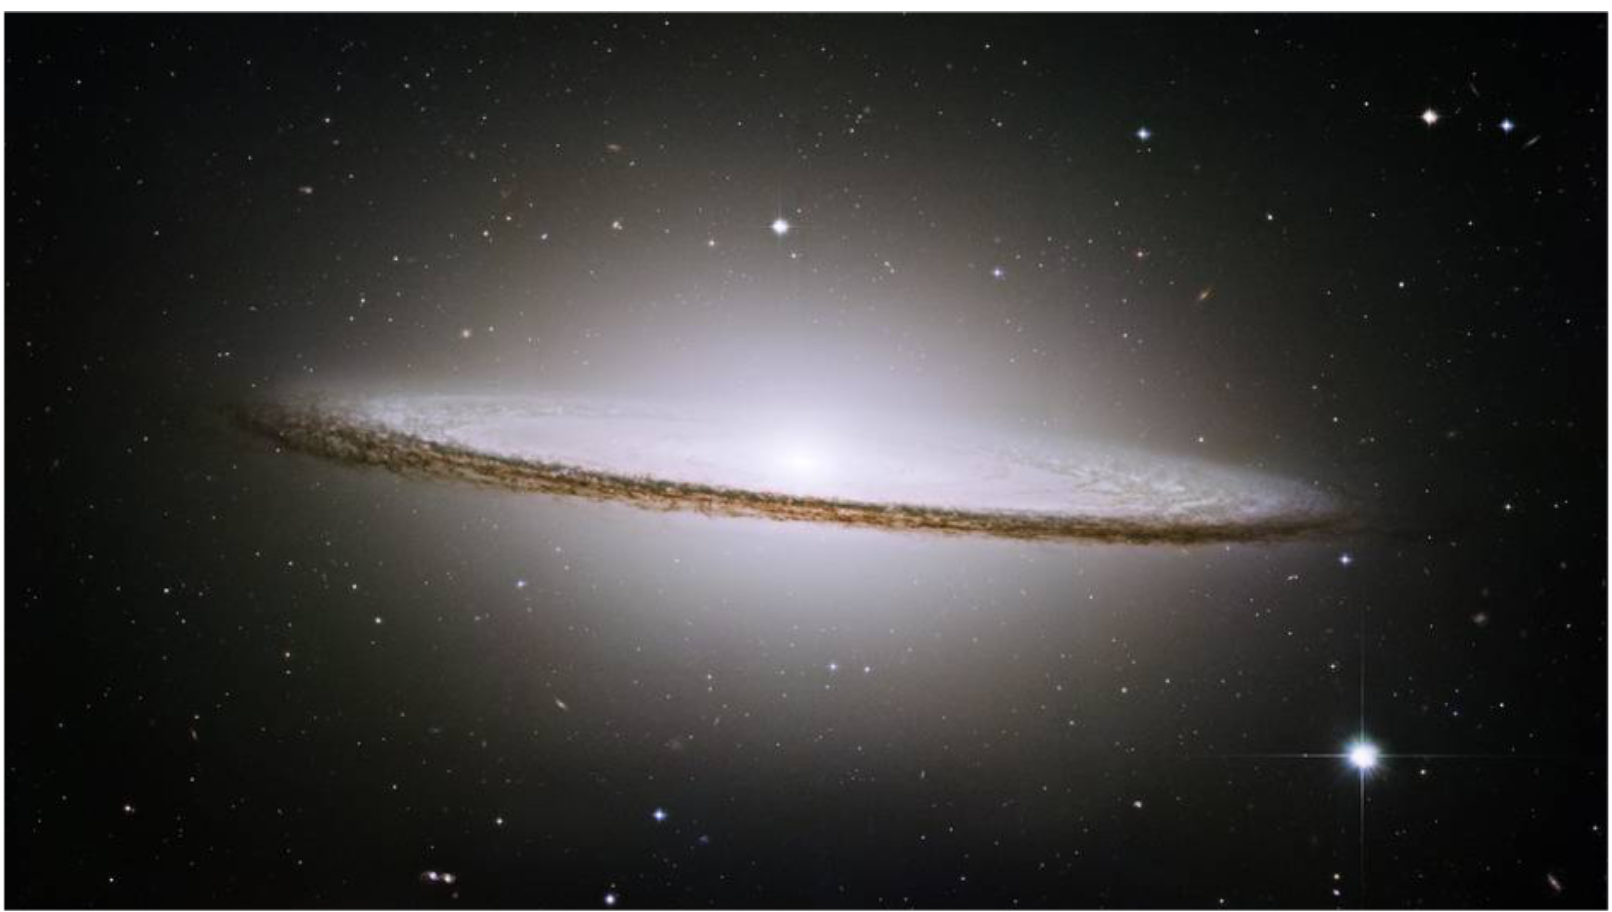
\includegraphics[width=1.0\linewidth]{disk_galaxy.png}
	\caption{典型的盘星系,盘面两侧亦有分布}
    \label{fig:disk}
\end{figure}

\begin{figure}[!hbtp]
	\centering 
	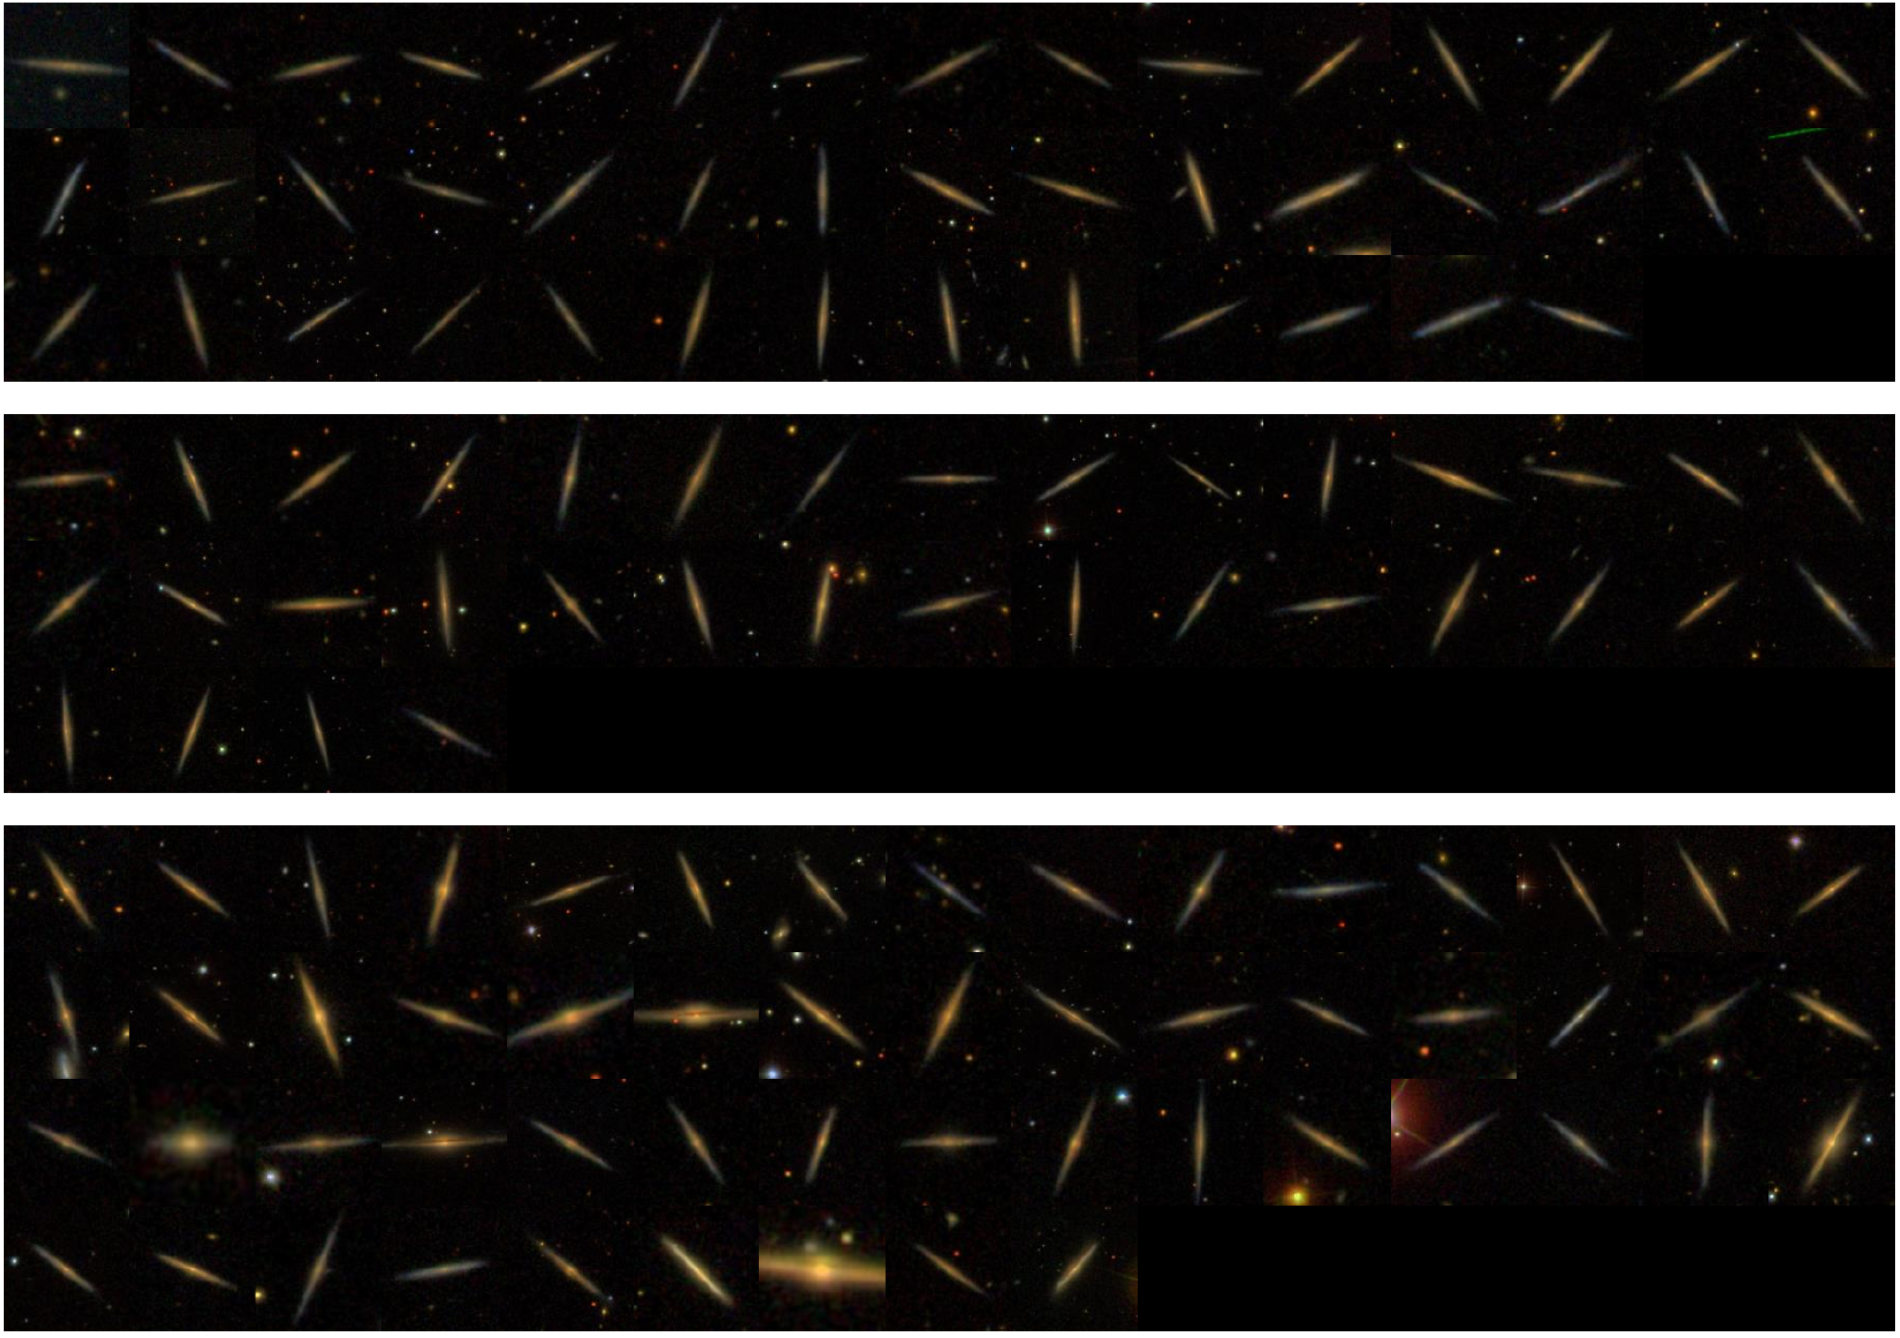
\includegraphics[width=1.0\linewidth]{pure_disk.png}
	\caption{只有盘的星系}
    \label{fig:pure-disk}
\end{figure}

盘星系的形成主要有以下步骤:
\begin{itemize}
    \item 气体落入暗物质晕,受到激波加热,形成暗物质晕中的一团热气体。
    \item 气体通过辐射冷却,降温后压强降低,气体团收缩。收缩中变热,经过几轮收缩和冷却后形成一团较密的气体团。
    \item 气体团不均匀收缩,各部分之间有相对运动,角动量逐渐转移集中,气体团开始整体性旋转。
    \item 角动量守恒让气体逐渐分布到盘上,面密度增加,密度足够高后形成恒星。
\end{itemize}

盘星系有以下统计特征:
\begin{itemize}
    \item 大的盘星系通常更亮。 如 \reffig{fig:Re-Mag} 所示。
    \item 越亮的盘星系通常更偏红。 如 \reffig{fig:red-Mag} 所示。
    \item 越亮的盘星系通常气体的占比更少。 如 \reffig{fig:gas-Mag} 所示。
    \item 越亮的盘星系转得越快, Tully-Fisher relation. (这个关系相对较明显。) 如 \reffig{fig:Tully-Fisher} 所示。
\end{itemize}

\begin{figure}[!hbtp]
	\centering 
    \subfigure[有效半径与绝对星等的关系]{
        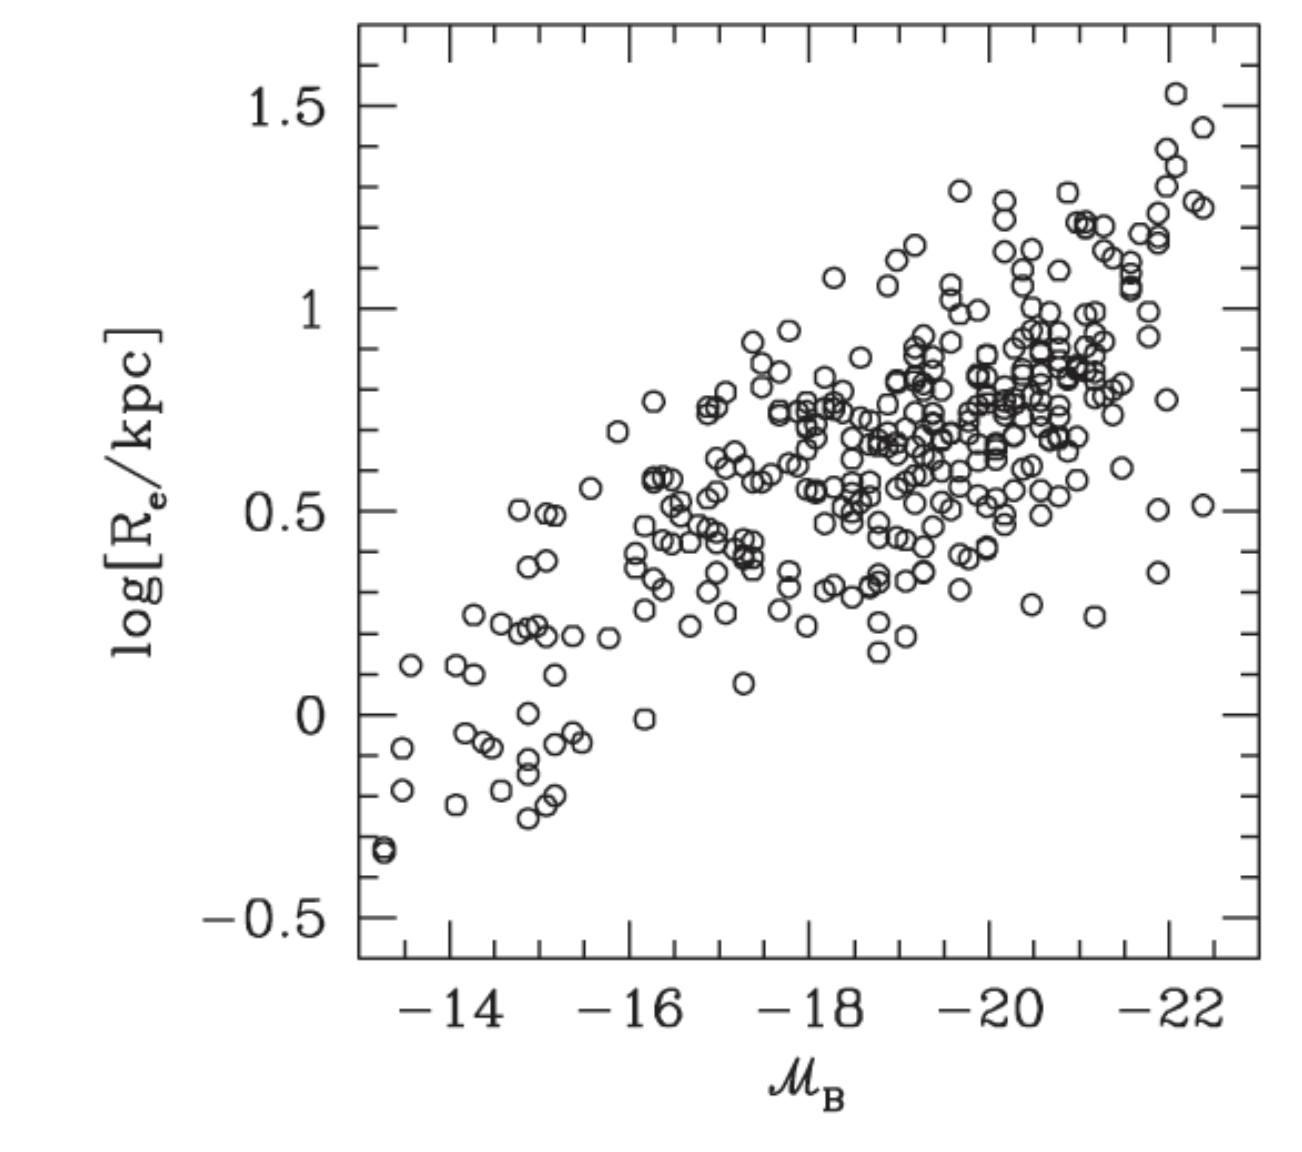
\includegraphics[width=0.4\linewidth]{Re-Mag.png}
        \label{fig:Re-Mag}
    }
    \quad
    \subfigure[色指数与绝对星等的关系]{
        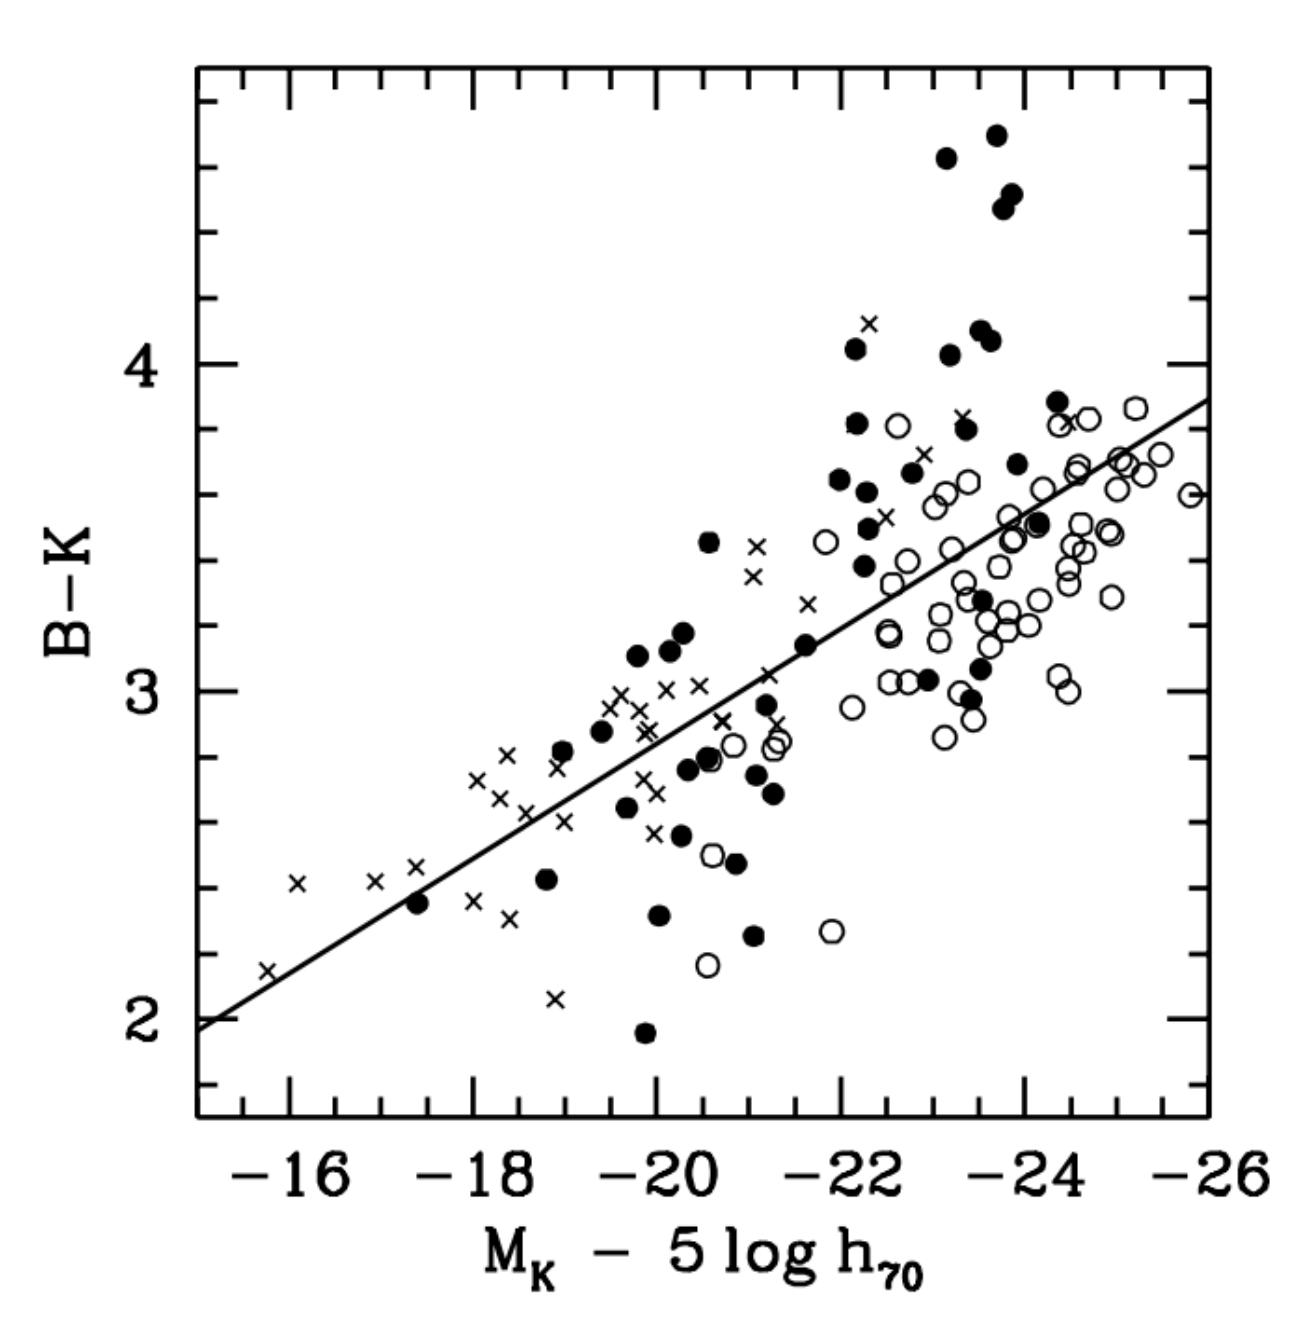
\includegraphics[width=0.4\linewidth]{red-Mag.png}
        \label{fig:red-Mag}
    }
	    
    \subfigure[气体占比与绝对星等的关系]{
        \includegraphics[width=0.4\linewidth]{gas-Mag.png}
        \label{fig:gas-Mag}
    }
    \quad	
    \subfigure[有效半径与绝对星等的关系]{
        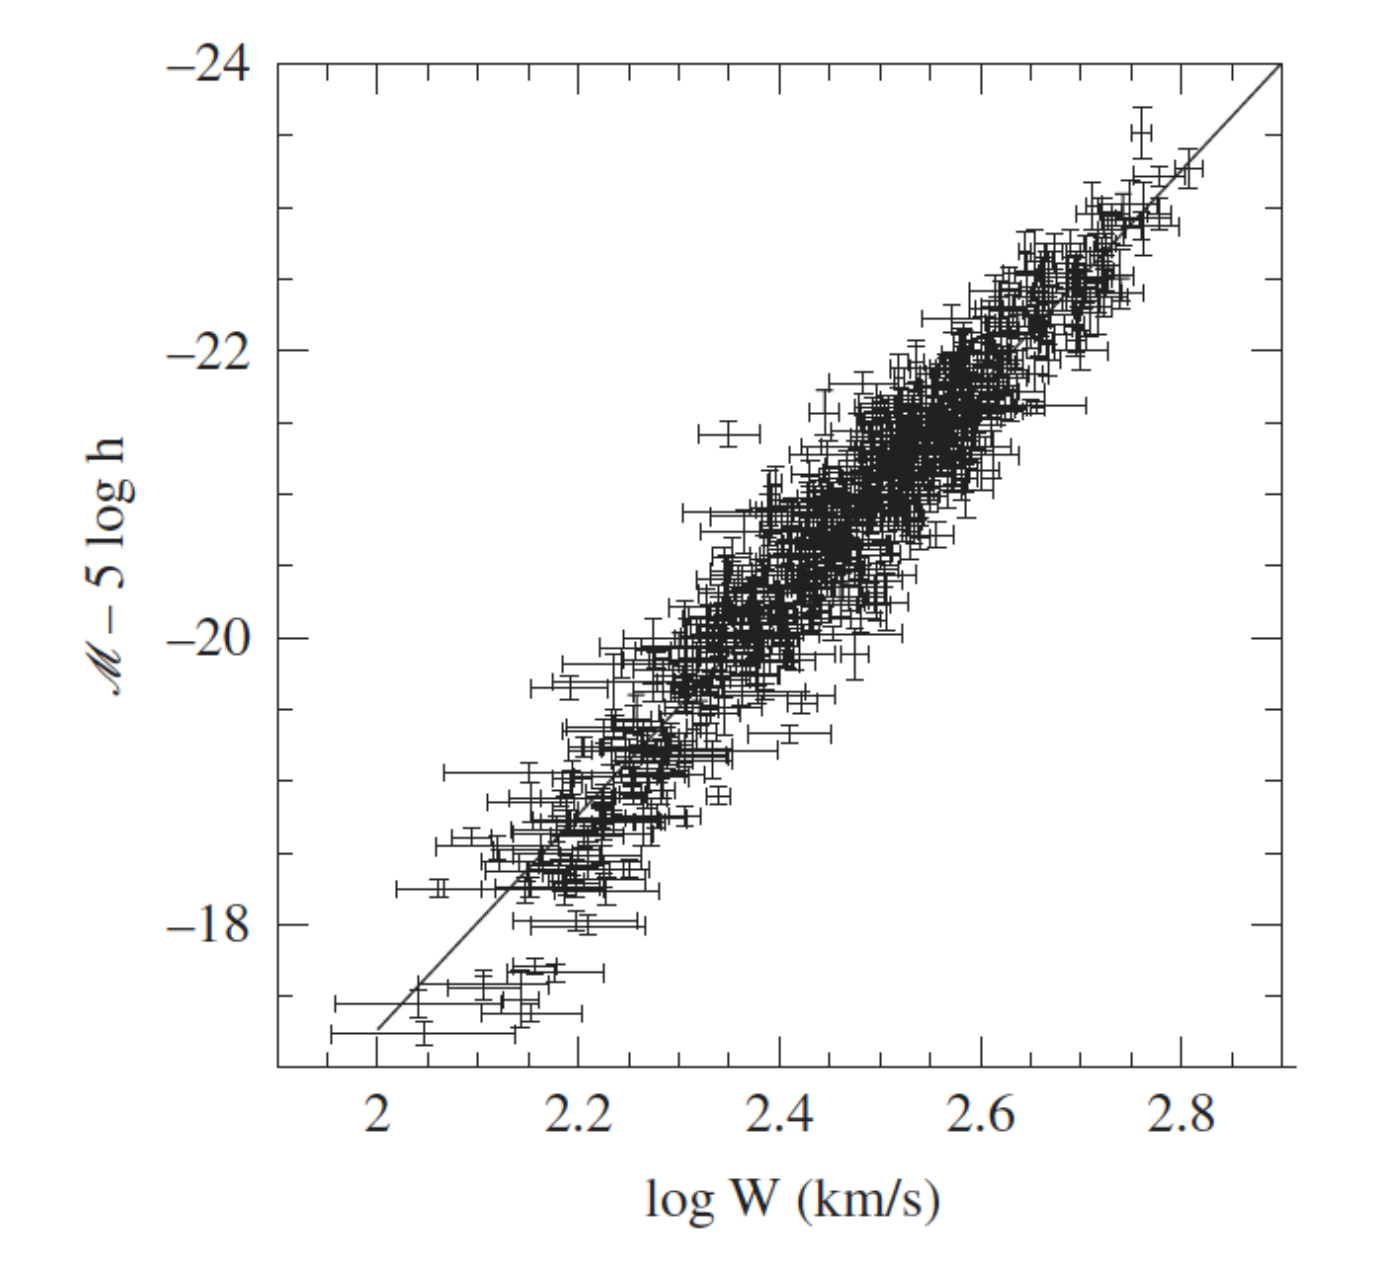
\includegraphics[width=0.4\linewidth]{TFrelation.png}
        \label{fig:Tully-Fisher}
    }
	
    \caption{盘星系的一些统计关系}
\end{figure}

\subsection{激波加热 (Shock heating)}

暗物质晕是维里化的。
气体在落入暗物质晕的过程中会与暗物质粒子相互作用,最终达到 $T _{\rm{sh}} $  温度。

假设初始气体的温度是可以忽略的,即 $v _{\rm{in}} ^2 \gg \frac{k_B T _{\rm{in}} }{\mu m_p}$.

初始能量是气体的动能 $E _{\rm{initial}} = \frac{1}{2} M _{\rm{gas}} v _{\rm{in}} ^2$

激波加热 $E _{\rm{sh}} = \frac{3}{2} N k_B T _{\rm{sh}} $
其中  $N=\frac{M _{\rm{gas}} }{\mu m_p}$ 是气体粒子的个数。

由 $E _{\rm{initial}} = E _{\rm{sh}} $,
得到 
$T _{\rm{sh}} =\frac{\mu m_p}{3k_B} v _{\rm{in}} ^2$.

对于暗物质晕来说 气体 $v _{\rm{in}} ^2 = \zeta v _{\rm{vir}} ^2$, $\zeta = \mathcal{O} (1)$ ,取决于 halo mass profile.

$T _{\rm{sh}} =\frac{\zeta \mu m_p}{3k_B} v _{\rm{vir}} ^2$


对于 被截断的奇异等温球 模型 (truncated, singular isothermal sphere of gas ),
$\zeta = 3/2$.

\begin{equation}
    T _{\rm{vir}} \equiv T _{\rm{sh}} = \frac{\mu m_p}{2k_B} v_{\rm{vir}} ^2 = 3.6\times 10^5 \mathrm{K} \left(\frac{ v_{\rm{vir}} }{100 \mathrm{~km/s}} \right) ^2
\end{equation}
定义为 维里温度。

维里温度是气体落入暗物质晕后被激波加热后所达到的温度,也用来标志一个暗物质晕可能孕育的星系在恒星形成前的气体温度。
所以,维里温度不是暗物质晕的温度,但是可以用来标志暗物质晕的性质。

\subsection{辐射冷却}

气体从高能级向低能级跃迁,辐射出光子带走能量,气体温度下降。具体的辐射机制较为复杂,本课暂不涉及。

\end{document}
